
\subsection{Simulation set-up}
In our experiment, the value of coefficients $b$ and $c$ in overhead functions (equation ~\ref{operationover} and ~\ref{intereferenceover}) are 0.05 and 1.5 respectively. The value of coefficient $\varphi$  in retention function (equation~\ref{eq:retention}) is 1. And the value of coefficients $\alpha$ and $\beta$ in utility function (equation~\ref{eq:reveneue})   are 100 and 60 respectively.
To demonstrate our proposal, the number of customers (i.e. number of VMs) ranges from 500 to 3000. 

We consider two types of datasets as described below:

\textit{Real Data Set:} Large dataset of a telephone company available at the Teradata Center at duke university\footnote{http://www.fuqua.duke.edu/} is used to compute real life churn rate (It is labeled as Telecom in our results). The dataset contains the information of more than 100000 customers. See Table~\ref{table1} for some sample features. We assume that data set for cloud service customers would be similar. 
 
\textit{Synthetic data:} Datasets representing various churn rates are generated by using Gaussian distribution function. We believe synthetic data represents variation of resource requests from users as observed in cloud computing industry.  


%\begin{table}[!h]
%\caption{Possible Cloud Customer Data (inspired by Telecom user dataset)}
%\label{table1}
%\centering
%\begin{tabular}{|p{2.4cm}|p{1.1cm}|p{2cm}|p{1.5cm}|}
%\hline
%\hline
%Features&Data type&Descrition&Example\\
%\hline
%\hline
%sbscrp\_id&number&customer ID&0019164958, 0019164958...\\
%\hline
%BIRTH\_DT&date&Date of birth&19610425, 19440112...\\
%\hline
%zip\_code&number&zip code&08648, 20774...\\
%\hline
%bill\_month&int&bills of customers&15219, 15249...\\
%\hline
%plan\_chosen&int&telephone plan&1, 2, 3, 4\\
%\hline
%total\_minute\_qty\_sum&int&total call minutes&57, 21...\\
%\hline
%churn&int&churner or non-churner&0, 1\\
%\hline
%\end{tabular}
%\end{table}

\begin{figure}[!h]
\centering
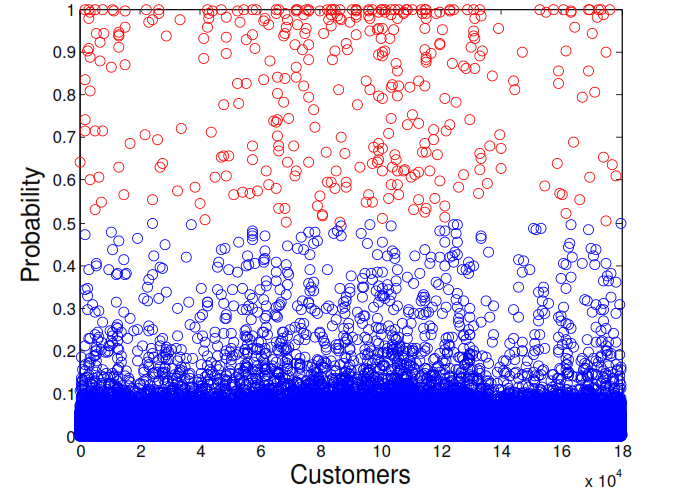
\includegraphics[scale = 0.52]{pic/churn.png}
\caption{ Churner (red bubbles) and non-churner (blue bubbles) identification in Telecom Data using naive bayesian method, churn rate = 3\%}
\label{Churnerclassification}
\end{figure}

\subsection{Results}

\subsubsection{Churner Classification} Naive Bayesian classifier is applied on Telecom dataset and result is shown in Figure~\ref{Churnerclassification}. Classifier is trained by using labeled data which is 10\% of the overall data set. We found Naive Bayesian classifier to be highly accurate. Moreover, using the classifier, churn rate in Telecom data is found to be 3\%. We believe cloud computing data would be similar to telecom customer data therefore, to demostrate our proposal on real data, we chose to  include results using Telecom data where different sample sizes are achieved by performing uniform sampling on the overall data. 

\subsubsection{Homogeneous VMs, Homogeneous PM}
In this scenario, all the requested VMs are same capacity of 0.2GHz. All PMs are of same capacity (= 3GHz, dual core) and they all costs the same (= 16).  Based on different churner rate, we use more PMs to give retention to large number of churners. Figure \ref{result1}(a) shows the number of PM used under various sizes of VMs (customers) for different churn rates. We observe a linear increase in number of PM used as number of VM increases. Small churn rates such as 0.03/0.05 can be handled by little to no increase in turned on PMs. However, for large churn rates more PMs need to be turned on. Figure \ref{result1}(b) shows the corresponding results on profit. Profit follows the similar trend where cloud service provide  
rs will have to sacrifice more revenue to tackle high churn rate.
\begin{figure*} [!htp]
  \centering
  \subfigure[Number of Physical Machines]{\label{outcastdroptail}
   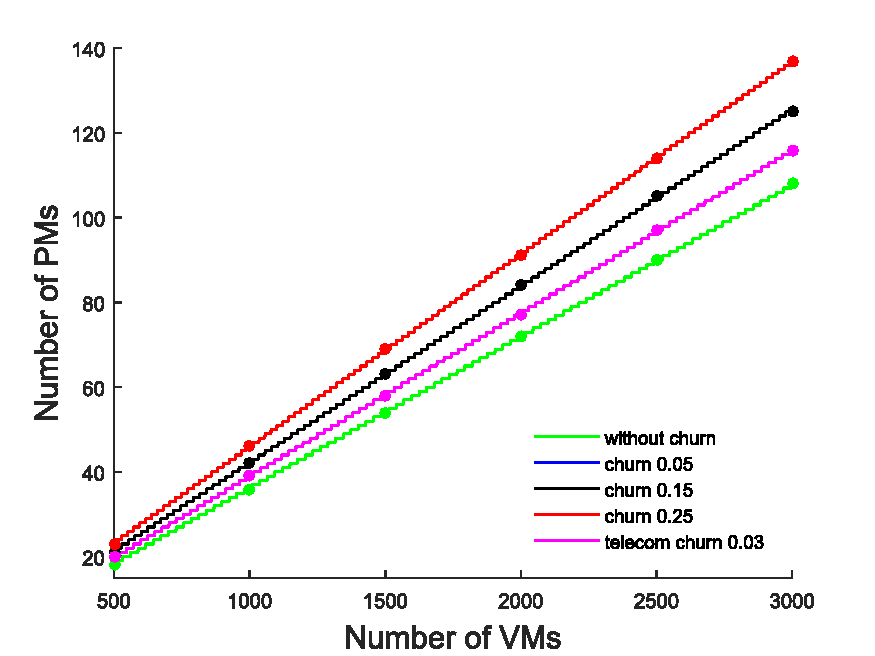
\includegraphics[width=0.4\textwidth]{pic/result1.pdf}} \quad
  \subfigure[Profit]{\label{outcastred}
   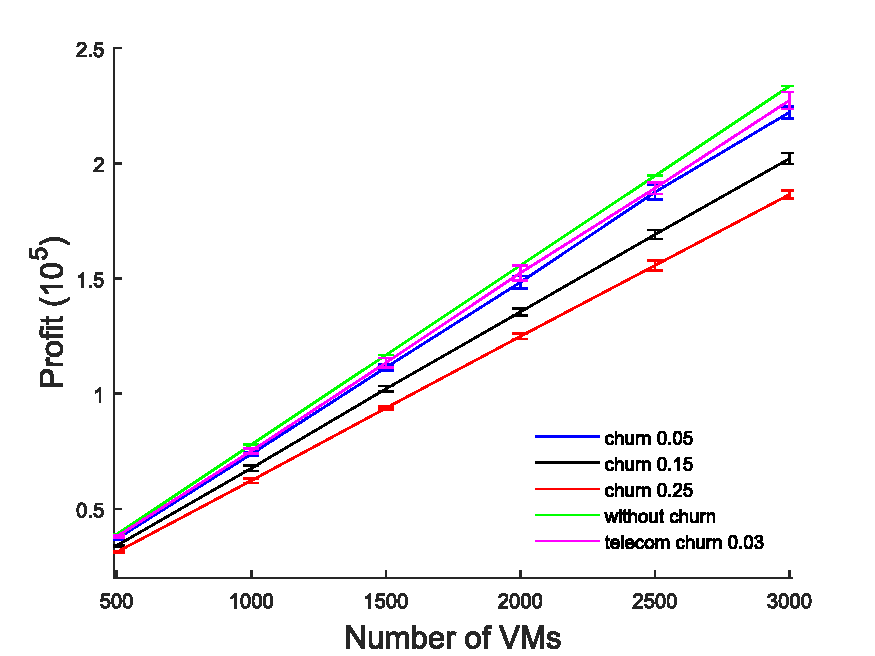
\includegraphics[width=0.4\textwidth]
{pic/profit1.pdf}} 
  \caption{Number of physical machines used and cloud service provider profit for homogeneous VMs (0.2GHz) and homogeneous PM (3GHz, dual core)  }
  \label{result1}
\end{figure*}


\subsubsection{Heterogeneous VMs, Homogeneous PMs}
In this scenario, all the requested VMs are of different capacities following a Gaussian distribution in capacity range from 0.25GHz to 1.5GHz whereas PMs are still the same as in the previous case. The trend in Figure~\ref{result2}(a) and Figure~\ref{result2}(b) is same as shown in previous section. However, because VMs request sizes have large variations, we observe profit has dropped significantly which is also evident by higher number of physical machine used as compared to previous case. Interestingly, we do not see an exact linear increase in either profit or number of PMs used as number of VM increases. The trend suggests that in the case of high number of customers, a little increase in customers with the same churn rate can be handled with little to no cost to the company. Results for churn and without churn show that such adaptation of the system is rooted in the integration of churn aware allocation and linear programming framework of VM placement. 

\begin{figure*} [!htp]
  \centering
  \subfigure[Number of Physical Machines]{\label{outcastdroptail}
   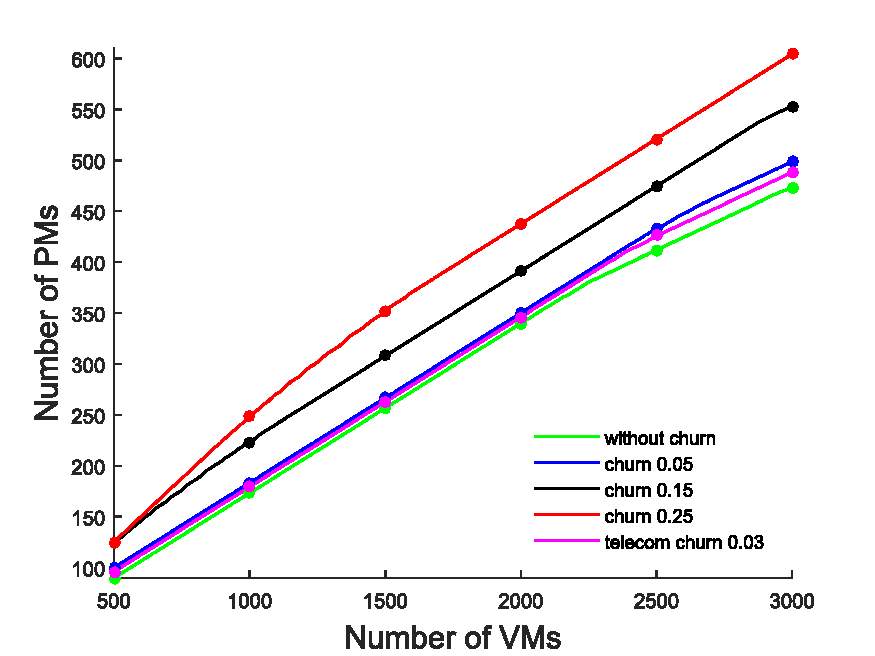
\includegraphics[width=0.4\textwidth]{pic/result2.pdf}} \quad
  \subfigure[Profit]{\label{outcastred}
   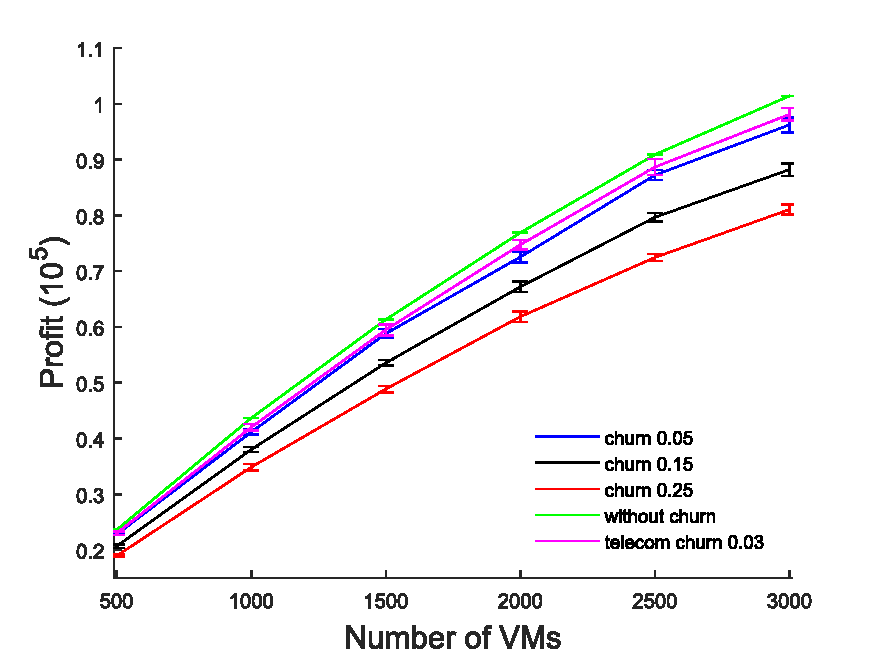
\includegraphics[width=0.4\textwidth]
{pic/profit2.pdf}} 
  \caption{ Number of physical machines used and cloud service provider profit for heterogeneous VMs and homogeneous PM (3GHz, dual core)  }
  \label{result2}
\end{figure*}


\begin{figure*} [!htp]
  \centering
  \subfigure[Number of Physical Machines]{\label{outcastdroptail}
   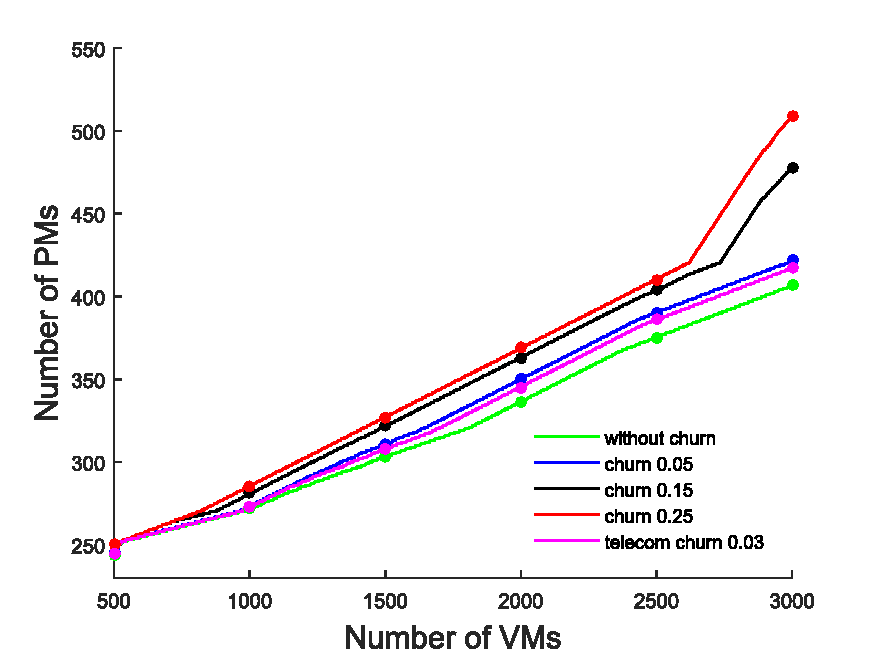
\includegraphics[width=0.4\textwidth]{pic/result3.pdf}} \quad
  \subfigure[Profit]{\label{outcastred}
   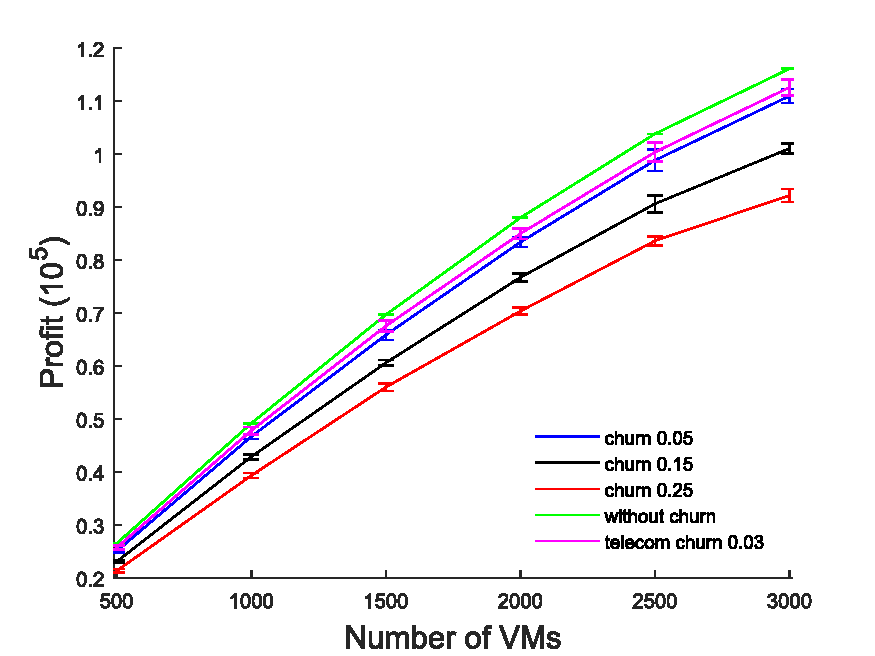
\includegraphics[width=0.4\textwidth]
{pic/profit3.pdf}} 
  \caption{ Number of physical machines used and cloud service provider profit for heterogeneous VMs and heterogeneous PMs  }
  \label{result3}
\end{figure*}

\subsubsection{Heterogeneous VMs, Heterogeneous PMs}
%Next case we considered the method to assign VMs into appropriate physical machines.The companies and service providers could have enough PMs for cloud computing, those PMs could be multifarious. For example, Amazon EC2 has many series physical infrastructures for cloud service, users can based their requirements to match and apply different VMs, some of them have strong CPU capacity for computing while some VMs are created with a low CPU capacity but a large hard disk space in order to store big data. Some service provider could have all same PMs and the VMs are also fixed. Based on section III, V and VI, we assume we have these PMs, and parameters in the below table \ref{table}. 

\begin{table}[!htp]
\caption{different Classes of Physical Machines used in the case of Heteregenous PMs}
\label{table}
\centering
\begin{tabular}{c|c|c|c|c}
\hline
\hline
Class&Capacity(GHz)& \# of Core &Cost& Machine count\\
\hline
\hline
A&3.0&8&100&20\\
\hline
B&2.7&6&85&30\\
\hline
C&2.5&6&70&50\\
\hline
D&3.0&4&60&100\\
\hline
E&2.5&4&55&150\\
\hline
F&2.5&2&40&200\\
\hline
G&2.0&2&20&200\\
\hline
H&1.5&2&10&250\\
\hline
\end{tabular}
\end{table}
The companies and service providers have PMs that are multifarious in nature to meet the diverse cloud customers. To simulate this scenario,  we use 8 classes of PMs and a total of 1000 PMs as shown in Table~\ref{table}. These PMs represent diverse capacity and costs found in a typical data centers (for example, Amazon EC2 has physical machines with diverse capacity and costs). The result for scenario is presented in Figure~\ref{result3}. The trend is similar as that of (Heterogeneous VMs, Heterogeneous PMs) case. However, we do observe a steep rise in number of PMs with the increase in VMs for higher churn rate, 0.15 and 0.25. The reason for this offshoot is with higher churn rate comes the more budget for retention action, therefore, higher added capacities for churners. Moreover, under this scheme, since machines with higher performance/cost runs out first the leftover machines being smaller in size putting a cap on number of VMs it can accommodate, therefore, we see a rise in number of machines used. However, profit trend is unaffected by it that reflects a good performance/cost ratio of machines in cloud datacenter. 

   

% An example of a floating table. Note that, for IEEE style tables, the 
% \caption command should come BEFORE the table. Table text will default to
% \footnotesize as IEEE normally uses this smaller font for tables.s
% The \label must come after \caption as always.
%


%Obviously, after the rank H has the highest Cost performance so we plan to use H fist, if Hs are not enough, then As come second, so on and so force until all VMs are placed on.
 %In our experiment,  Then, we use two algorithms for these 3000 VMs to place on 1000 PMs, the result is shown in figure x.
 





